\documentclass[../../main.tex]{subfiles}
\graphicspath{{../../image/}{../../figure/}}
\begin{document}

\section{证据下界}\label{section:ch16-证据下界}

在讨论离散潜变量模型时，我们推导出了边缘对数似然的证据下界（ELBO），并展示了它是如何构成期望最大化（EM）算法的基础的。相同的框架同样适用于连续潜变量模型。这里我们提供一个稍微不同的~ELBO~推导，并且假设潜变量 $\bm{z}$ 是连续的。

考虑一个带有观测变量 $\bm{x}$、潜变量 $\bm{z}$ 和可学习参数向量 $\bm{w}$ 的模型 $p(\bm{x},\bm{z}|\bm{w})$。只要引入潜变量上的任意一个分布 $q(\bm{z})$，我们就可以将对数似然函数 $\ln p(\bm{x}|\bm{w})$ 写成两项之和的形式：
\begin{align}
\ln p(\bm{x}|\bm{w})=\mathcal{L}(q,\bm{w})+\operatorname{KL}\!\left(q(\bm{z})\,\|\,p(\bm{z}|\bm{x},\bm{w})\right)
\label{align:ch16-elbo}
\end{align}
其中
\begin{align}
\mathcal{L}(q,\bm{w})=\int q(\bm{z})\ln\!\left\{\frac{p(\bm{x},\bm{z}|\bm{w})}{q(\bm{z})}\right\}\mathrm{d}\bm{z}
\label{align:ch16-elbo-def}
\end{align}
而
\begin{align}
\operatorname{KL}\!\left(q(\bm{z})\,\|\,p(\bm{z}|\bm{x},\bm{w})\right)=-\int q(\bm{z})\ln\!\left\{\frac{p(\bm{z}|\bm{x},\bm{w})}{q(\bm{z})}\right\}\mathrm{d}\bm{z}.
\label{align:ch16-kl}
\end{align}

$\operatorname{KL}(q\|p)$ 是一种~Kullback--Leibler~散度，满足 $\operatorname{KL}(q\|p)\geq 0$，从中可以得出
\begin{align}
\ln p(\bm{x}|\bm{w})\geq\mathcal{L}(q,\bm{w})
\label{align:ch16-elbo-ineq}
\end{align}
式\eqref{align:ch16-elbo-def}给出的 $\mathcal{L}(q,\bm{w})$ 构成了对数似然的下界，称为证据下界（ELBO）。

我们可以使用~EM~算法的两阶段迭代过程来最大化对数似然函数。在~EM~算法中，我们交替地针对 $q(\bm{z})$（E~步骤）和 $\bm{w}$（M~步骤）最大化 $\mathcal{L}(q,\bm{w})$。首先初始化参数 $\bm{w}$。然后在~E~步骤中保持 $\bm{w}$ 固定，并针对 $q(\bm{z})$ 最大化下界。我们注意到，可以通过最小化式\eqref{align:ch16-kl}中的~Kullback--Leibler~散度来获得下界的最高值。换言之，当~Kullback--Leibler~散度为零时，$q(\bm{z})=p(\bm{z}|\bm{x},\bm{w})$。

在~M~步骤中，我们保持所选的 $q(\bm{z})$ 固定，并针对 $\bm{w}$ 最大化 $\mathcal{L}(q,\bm{w})$。将 $q(\bm{z})=p(\bm{z}|\bm{x},\bm{w}^{\text{old}})$ 代入式\eqref{align:ch16-elbo-def}，可以得到
\begin{align}
\mathcal{L}(q,\bm{w})=\int p(\bm{z}|\bm{x},\bm{w}^{\text{old}})\ln p(\bm{x},\bm{z}|\bm{w})\,\mathrm{d}\bm{z}-\int p(\bm{z}|\bm{x},\bm{w}^{\text{old}})\ln p(\bm{z}|\bm{x},\bm{w}^{\text{old}})\,\mathrm{d}\bm{z}.
\label{align:ch16-q-continuous}
\end{align}

右侧的第二项独立于 $\bm{w}$，因此在~M~步骤中可以忽略。式\eqref{align:ch16-q-continuous}右侧的第一项则是完整数据对数似然的期望，该期望来自我们用 $\bm{w}^{\text{old}}$ 计算得到的 $\bm{z}$ 的后验分布。

如果我们有一个由独立同分布观测值组成的数据集 $\bm{x}_1,\cdots,\bm{x}_N$，则似然函数的形式为
\begin{align}
\ln p(\bm{X}|\bm{w})=\sum_{n=1}^{N}\ln p(\bm{x}_n|\bm{w})
\label{align:ch16-iid-nll}
\end{align}
其中数据矩阵 $\bm{X}$ 包含 $\bm{x}_1,\cdots,\bm{x}_N$，并且参数 $\bm{w}$ 在所有数据点之间是共享的。对于每一个数据点，引入一个相应的潜变量 $\bm{z}_n$ 及其关联的分布 $q(\bm{z}_n)$，并且通过遵循类似于推导式\eqref{align:ch16-elbo}时使用的步骤，我们得到了以下形式的~ELBO：
\begin{align}
\mathcal{L}(q,\bm{w})=\sum_{n=1}^{N}\int q(\bm{z}_n)\ln p(\bm{x}_n,\bm{z}_n|\bm{w})\,\mathrm{d}\bm{z}_n-\sum_{n=1}^{N}\int q(\bm{z}_n)\ln q(\bm{z}_n)\,\mathrm{d}\bm{z}_n.
\label{align:ch16-elbo-iid}
\end{align}

当讨论变分自编码器（见第~19~章）时，我们将遇到一个模型，其~E~步骤的精确解无法实现，因此我们改为使用深度神经网络对 $q(\bm{z})$ 进行建模，然后使用~ELBO~来学习网络的参数。

\subsection{EM算法}\label{subsection:ch16-em算法}

我们可以按照~EM~算法的通用框架来导出概率~PCA~的~EM~算法。为此，我们写下完整数据对数似然函数并根据用"旧"参数值评估的潜变量分布的后验分布来获取期望，然后最大化这个完整数据对数似然函数的期望以产生"新"的参数值。因为我们假定数据点是独立的，所以完整数据对数似然函数的形式为
\begin{align}
\ln p(\bm{X},\bm{Z}|\bm{W},\bm{\mu},\sigma^2)=-\frac{ND}{2}\ln(2\pi\sigma^2)-\frac{1}{2\sigma^2}\sum_{n=1}^{N}\|\bm{x}_n-\bm{\mu}-\bm{W}\bm{z}_n\|^2-\frac{N}{2}\ln(2\pi)-\frac{1}{2}\sum_{n=1}^{N}\|\bm{z}_n\|^2
\label{align:ch16-complete-nll}
\end{align}
其中矩阵 $\bm{Z}$ 的第 $n$ 行由 $\bm{z}_n^{\mathsf T}$ 给出。我们已经知道 $\bm{\mu}$ 的精确最大似然解是由样本均值 $\bar{\bm{x}}$[式\eqref{align:ch16-mean}]给出的，在这个阶段替代 $\bm{\mu}$ 是很方便的。利用式\eqref{align:ch16-prior-z}和式\eqref{align:ch16-conditional-x}所示的潜变量分布和条件分布，并且考虑到对潜变量的后验分布的期望，我们得到
\begin{align}
\mathbb{E}_{\bm{Z}}\!\left[\ln p(\bm{X},\bm{Z}|\bm{W},\sigma^2)\right]=-\frac{ND}{2}\ln(2\pi\sigma^2)-\frac{1}{2\sigma^2}\sum_{n=1}^{N}\left\{\|\bm{x}_n-\bar{\bm{x}}\|^2-2(\bm{x}_n-\bar{\bm{x}})^{\mathsf T}\bm{W}\mathbb{E}[\bm{z}_n]+\operatorname{tr}(\bm{W}^{\mathsf T}\bm{W}\,\mathbb{E}[\bm{z}_n\bm{z}_n^{\mathsf T}])\right\}-\frac{1}{2}\sum_{n=1}^{N}\mathbb{E}[\bm{z}_n^{\mathsf T}\bm{z}_n]+\text{常数}.
\label{align:ch16-q-ppca}
\end{align}

注意，此情况仅通过高斯分布的充分统计量与后验分布产生关联。因此，在~E~步骤中，我们使用旧的参数值来计算期望：
\begin{align}
\mathbb{E}[\bm{z}_n]=\bm{M}^{-1}\bm{W}^{\mathsf T}(\bm{x}_n-\bar{\bm{x}})
\label{align:ch16-e-step-z}
\end{align}
\begin{align}
\mathbb{E}[\bm{z}_n\bm{z}_n^{\mathsf T}]=\sigma^2\bm{M}^{-1}+\mathbb{E}[\bm{z}_n]\mathbb{E}[\bm{z}_n]^{\mathsf T}
\label{align:ch16-e-step-zz}
\end{align}
这里的 $\bm{M}$ 由式\eqref{align:ch16-matrix-m}定义。以上这些可以直接从后验分布和标准结果 $\mathbb{E}[\bm{z}_n\bm{z}_n^{\mathsf T}]=\operatorname{cov}[\bm{z}_n]+\mathbb{E}[\bm{z}_n]\mathbb{E}[\bm{z}_n]^{\mathsf T}$ 中得出。

在~M~步骤中，我们固定后验统计量，并针对 $\bm{W}$ 和 $\sigma^2$ 进行最大化。针对 $\sigma^2$ 的最大化相对简单，针对 $\bm{W}$ 的最大化则需要我们利用矩阵导数获得~M~步骤的如下方程：
\begin{align}
\bm{W}^{\text{new}}=\left[\sum_{n=1}^{N}(\bm{x}_n-\bar{\bm{x}})\mathbb{E}[\bm{z}_n]^{\mathsf T}\right]\left[\sum_{n=1}^{N}\mathbb{E}[\bm{z}_n\bm{z}_n^{\mathsf T}]\right]^{-1}
\label{align:ch16-m-step-w}
\end{align}
\begin{align}
(\sigma^2)^{\text{new}}=\frac{1}{ND}\sum_{n=1}^{N}\left\{\|\bm{x}_n-\bar{\bm{x}}\|^2-2(\bm{x}_n-\bar{\bm{x}})^{\mathsf T}\bm{W}^{\text{new}}\mathbb{E}[\bm{z}_n]+\operatorname{tr}(\bm{W}^{\text{new}\mathsf T}\bm{W}^{\text{new}}\,\mathbb{E}[\bm{z}_n\bm{z}_n^{\mathsf T}])\right\}.
\label{align:ch16-m-step-sigma}
\end{align}

概率~PCA~的~EM~算法将首先初始化参数，然后交替地在~E~步骤中使用式\eqref{align:ch16-e-step-z}和式\eqref{align:ch16-e-step-zz}计算潜空间后验分布的充分统计量，并在~M~步骤中使用式\eqref{align:ch16-m-step-w}和式\eqref{align:ch16-m-step-sigma}修正参数值。

概率~PCA~的~EM~算法的一个好处是，其在大规模应用中的计算效率较高。与基于样本协方差矩阵的特征向量分解的传统~PCA~不同，~EM~算法是迭代的。传统~PCA~的计算效率要高得多：协方差矩阵的特征分解需要 $O(D^3)$ 次计算。通常我们只对前 $M$ 个特征向量及对应的特征值感兴趣，在这种情况下，我们可以使用计算成本仅为 $O(MD^2)$ 的算法。然而，计算协方差矩阵需要 $O(ND^2)$ 的计算成本。这里描述的~EM~算法也没有显式构造协方差矩阵。计算最密集的步骤涉及数据集的求和，其复杂度为 $O(NDM)$。对于很大的维度 $D$，$M$ 要远小于 $D$，与 $O(ND^2)$ 相比，这可以显著节省计算成本。

\subsection{PCA的EM算法}\label{subsection:ch16-pca-em}

EM~算法的另一个优雅特性是，我们可以取极限 $\sigma^2\rightarrow 0$，这对应于传统~PCA，并且仍然是一个有效的类~EM~算法。从式\eqref{align:ch16-e-step-z}中可以看到，在~E~步骤中唯一需要计算的量是 $\mathbb{E}[\bm{z}_n]$。此外，因为 $\bm{M}=\bm{W}^{\mathsf T}\bm{W}$，所以~M~步骤也简化了。为了强调算法的简洁性，定义 $\tilde{\bm{X}}$ 为一个大小为 $N\times D$ 的矩阵，其第 $n$ 行由向量 $(\bm{x}_n-\bar{\bm{x}})^{\mathsf T}$ 给出。类似地，定义 $\bm{\Omega}$ 为一个大小为 $M\times N$ 的矩阵，其第 $n$ 列由 $\mathbb{E}[\bm{z}_n]$ 给出。~PCA~的~EM~算法的~E~步骤变为
\begin{align}
\bm{\Omega}=(\bm{W}^{\mathsf T}\bm{W})^{-1}\bm{W}^{\mathsf T}\tilde{\bm{X}}^{\mathsf T}
\label{align:ch16-pca-e}
\end{align}
EM~算法的~M~步骤变为
\begin{align}
\bm{W}^{\text{new}}=\tilde{\bm{X}}^{\mathsf T}\bm{\Omega}^{\mathsf T}(\bm{\Omega}\bm{\Omega}^{\mathsf T})^{-1}.
\label{align:ch16-pca-m}
\end{align}

\begin{figure}[htbp]
\centering
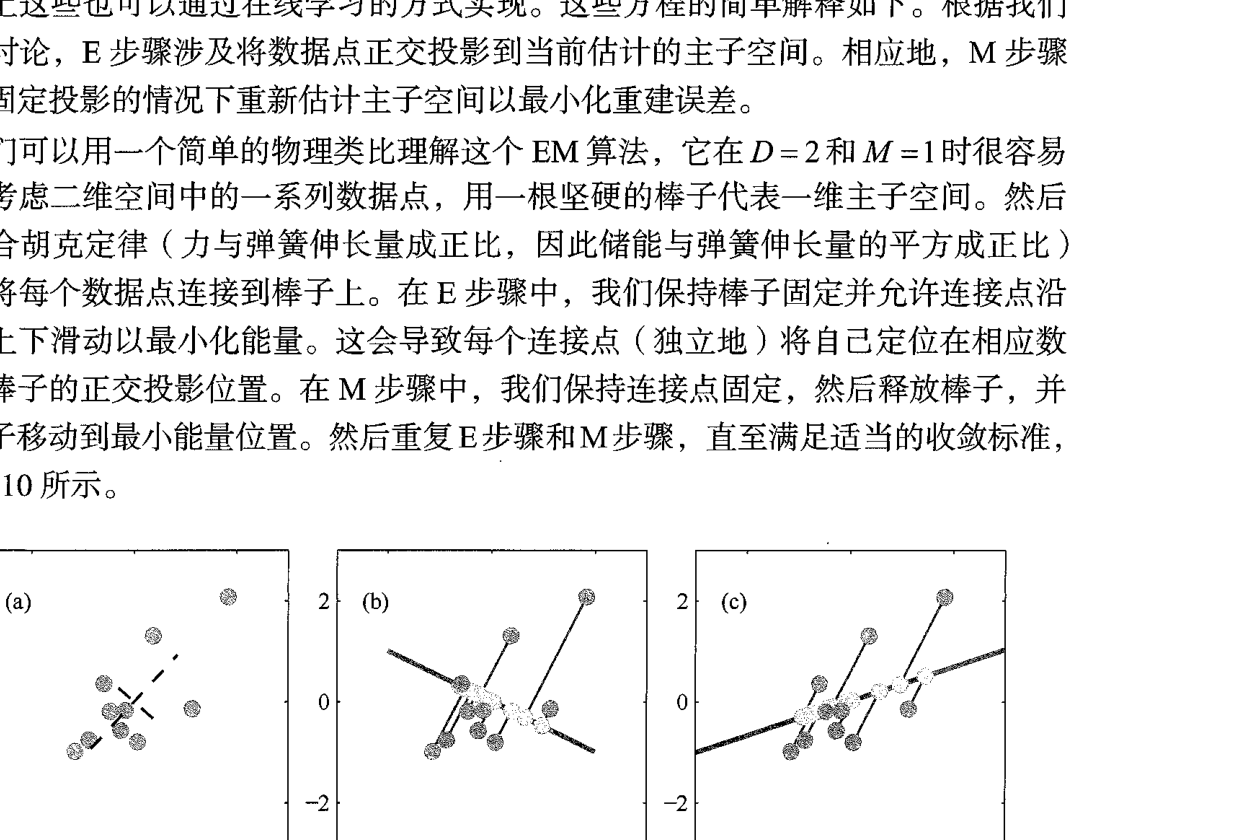
\includegraphics[width=0.9\textwidth]{ch16-fig16.10-em-spring.png}
\caption{用一个简单的物理类比来说明~PCA~的~EM~算法。(a)~一组绿色的数据点以及真实的主成分（显示为按特征值平方根缩放的特征向量）；(b)~由 $\bm{W}$ 定义的主子空间的初始配置（显示为红色），以及潜在点 $\bm{Z}$ 在数据空间中的投影（由 $\bm{Z}\bm{W}^{\mathsf T}$ 给出，显示为青色）；(c)~经过第一个~M~步骤后，$\bm{W}$ 已经在 $\bm{Z}$ 保持固定的情况下得到更新；(d)~在随后的~E~步骤中，$\bm{Z}$ 的值已更新并给出了正交投影，并且 $\bm{W}$ 保持不变；(e)~经过第二个~M~步骤之后的结果；(f)~收敛后的解。}
\label{fig:ch16-em-spring}
\end{figure}

我们可以用一个简单的物理类比理解这个~EM~算法，它在 $D=2$ 和 $M=1$ 时很容易描绘。考虑二维空间中的一系列数据点，用一根坚硬的棒子代表一维主子空间。然后通过符合胡克定律（力与弹簧伸长量成正比，因此储能与弹簧伸长量的平方成正比）的弹簧将每个数据点连接到棒子上。在~E~步骤中，我们保持棒子固定并允许连接点沿着棒子上下滑动以最小化能量。这会导致每个连接点（独立地）将自己定位在相应数据点到棒子的正交投影位置。在~M~步骤中，我们保持连接点固定，然后释放棒子，并允许棒子移动到最小能量位置。然后重复~E~步骤和~M~步骤，直至满足适当的收敛标准。

以上这些也可以通过在线学习的方式实现。这些方程的简单解释如下：根据我们之前的讨论，E~步骤涉及将数据点正交投影到当前估计的主子空间。相应地，M~步骤表示在固定投影的情况下重新估计主子空间以最小化重建误差。

\subsection{因子分析的EM算法}\label{subsection:ch16-fa-em}

我们可以使用最大似然法来确定因子分析模型中的参数 $\bm{\mu}$、$\bm{W}$ 和 $\bm{\Psi}$。$\bm{\mu}$ 的解再次由样本均值给出。然而，与概率~PCA~不同的是，$\bm{W}$ 不再有闭式的最大似然解，只能通过迭代来找到。由于因子分析模型是一个潜变量模型，因此可以使用类似于概率~PCA~的~EM~算法来完成这项工作。具体来说，E~步骤方程为
\begin{align}
\mathbb{E}[\bm{z}_n]=\bm{G}\bm{W}^{\mathsf T}\tilde{\bm{X}}_n^{-1}(\bm{x}_n-\bar{\bm{x}})
\label{align:ch16-fa-e-z}
\end{align}
\begin{align}
\mathbb{E}[\bm{z}_n\bm{z}_n^{\mathsf T}]=\bm{G}+\mathbb{E}[\bm{z}_n]\mathbb{E}[\bm{z}_n]^{\mathsf T}
\label{align:ch16-fa-e-zz}
\end{align}
其中
\begin{align}
\bm{G}=(\bm{I}+\bm{W}^{\mathsf T}\bm{\Psi}^{-1}\bm{W})^{-1}
\label{align:ch16-fa-g}
\end{align}
注意这是以一种涉及对 $M\times M$ 而不是 $D\times D$ 的矩阵（除了 $D\times D$ 对角矩阵，其逆在 $O(D)$ 步内可以轻松计算）求逆的形式来表示的，这很方便，因为通常情况下 $M<D$。

同样，M~步骤方程为
\begin{align}
\bm{W}^{\text{new}}=\left[\sum_{n=1}^{N}(\bm{x}_n-\bar{\bm{x}})\mathbb{E}[\bm{z}_n]^{\mathsf T}\right]\left[\sum_{n=1}^{N}\mathbb{E}[\bm{z}_n\bm{z}_n^{\mathsf T}]\right]^{-1}
\label{align:ch16-fa-m-w}
\end{align}
\begin{align}
\bm{\Psi}^{\text{new}}=\operatorname{diag}\!\left\{\tilde{\bm{S}}-\frac{1}{N}\sum_{n=1}^{N}(\bm{x}_n-\bar{\bm{x}})\mathbb{E}[\bm{z}_n]^{\mathsf T}\bm{W}^{\text{new}\mathsf T}\right\}
\label{align:ch16-fa-m-psi}
\end{align}
其中 $\operatorname{diag}$ 运算符会将矩阵的所有非对角元素设置为零。

\end{document}
